\documentclass[svgnames,dvipsnames,hyperref={bookmarks=false},usepdftitle=false]{beamer}
\usetheme{scaladays}

\title{Easy Metaprogramming For Everyone!}
\author{Eugene Burmako (\href{https://twitter.com/xeno_by}{@xeno{\textunderscore}by})\\ Denys Shabalin (\href{https://twitter.com/den_sh}{@den\_sh})}
\institute{\'Ecole Polytechnique F\'ed\'erale de Lausanne \\ \texttt{http://scalameta.org/}}
\date{17 June 2014}
\hypersetup{pdfauthor={Eugene Burmako, Denys Shabalin},pdftitle={Easy Metaprogramming For Everyone!}}

\begin{document}

\titleframe

\begin{frame}{Metaprogramming is...}
\begin{quote}
Metaprogramming is the writing of computer programs that write or manipulate other programs or themselves as their data.
\end{quote}
\begin{flushright}
\textemdash Wikipedia
\end{flushright}
\end{frame}

% TODO: give some examples in \begin{web}...\end{web}
\begin{frame}{Metaprogramming is useful}
\begin{itemize}
\item Code generation
\item Program verification
\item Style checking
\item Refactoring
\item Incremental compilation
\item Documentation generation
\item ...
\end{itemize}
\end{frame}

\begin{frame}[c, fragile]{Before Scala 2.10}
\begin{center}
% http://completenostalgia.com/transport/
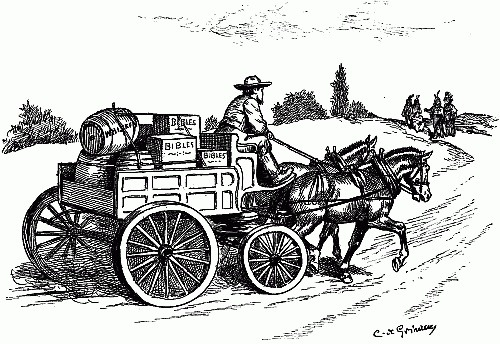
\includegraphics[height=7cm]{horse.jpg}
\end{center}
\end{frame}

\begin{frame}{Baby steps of Scala metaprogramming}
\begin{itemize}
\item Text-based introspection with scalap
\item Unstable and undocumented compiler plugins
\item Ad-hoc textual code generation
\end{itemize}
\end{frame}

\begin{frame}[c, fragile]{After Scala 2.10}
\begin{center}
% https://www.autocad360.com/blog/wp-content/uploads/2011/05/ford-model-t_141.jpg
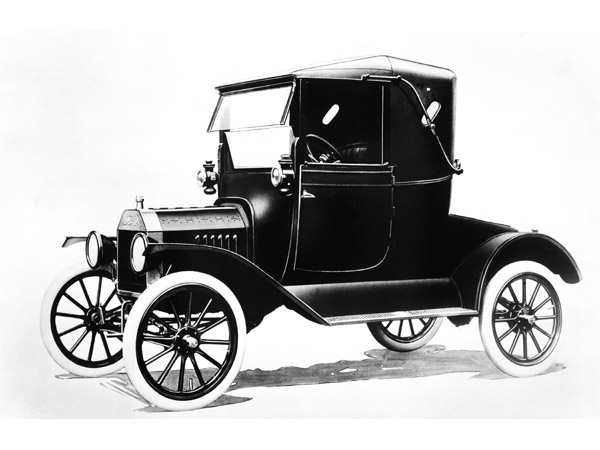
\includegraphics[height=7cm]{car.jpg}
\end{center}
\end{frame}

\begin{frame}{Current state of things}
Metaprogramming with \texttt{scala.reflect}:
\begin{itemize}
\item[+] Full-fledged model of Scala available in standard distribution
\item[+] Structured code generation with macros and quasiquotes
\end{itemize}
\pause
\begin{itemize}
\item[\textendash] Complicated: optimized towards compiler developers, not library users
\item[\textendash] Brittle: a lot of unspecified and hard-to-satisfy invariants
\item[\textendash] Locked-in: tightly bound to \texttt{scalac} internals
\end{itemize}
\end{frame}

\begin{frame}{Nevertheless \texttt{scala.reflect} has proven to be useful}
\begin{itemize}
\item Enables libraries like \texttt{async}, \texttt{pickling}, \texttt{scala-blitz}, etc
\item Empowers existing solutions in \texttt{scalatest}, \texttt{Play!}, \texttt{parboiled}, etc
\item Foundation for high-level abstractions: \texttt{shapeless}, \texttt{yin-yang}, etc
\end{itemize}
\end{frame}

\begin{frame}[c, fragile]{We are building an even better tech}
\begin{center}
% http://www.utopiaplanitia.info/blueprints.html
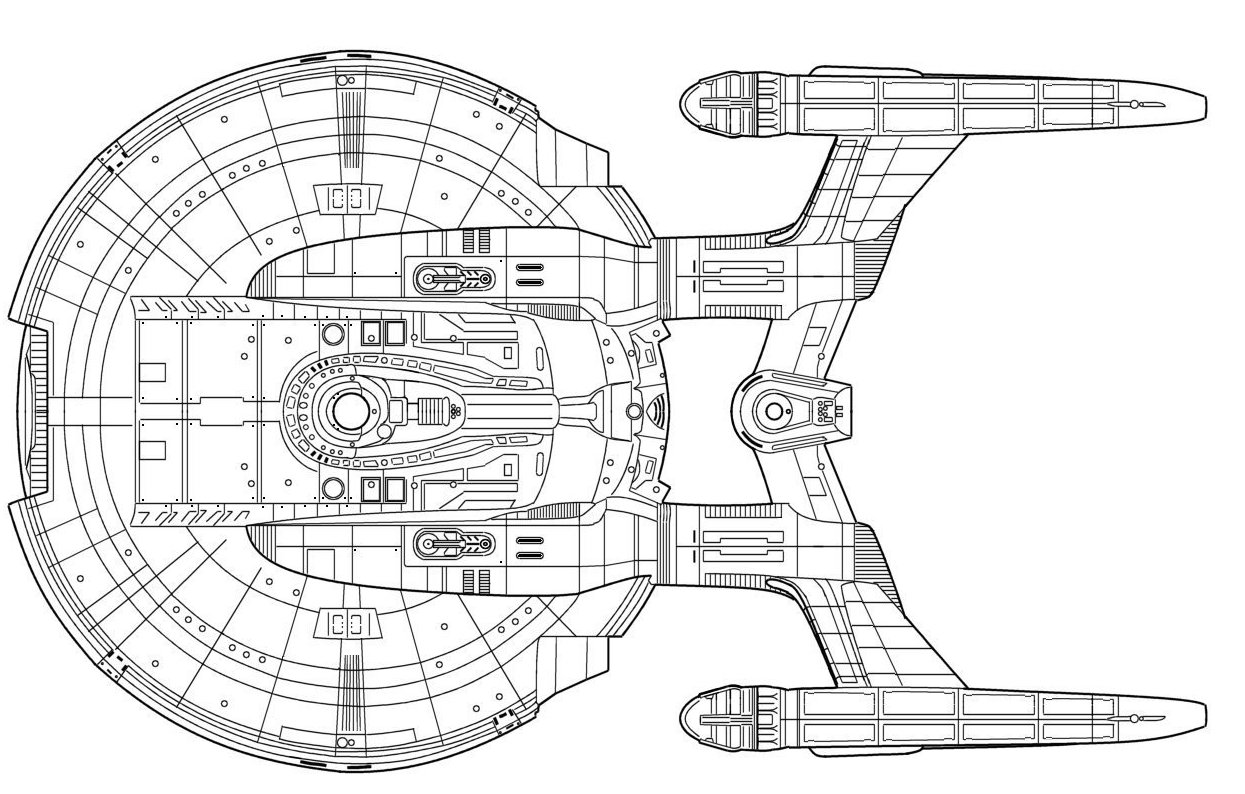
\includegraphics[height=7.5cm]{nx01-wireframe.jpg}
\end{center}
\end{frame}

% TODO: the scala.meta hype train is leaving the station
% \begin{frame}
% \vskip40pt
% \begin{center}
% \text{\color{black}\LARGE{scala\visible<2>{.}meta\visible<1>{programming}}}
% \end{center}
% \end{frame}

\begin{frame}{Meet our new metaprogramming platform}
\begin{itemize}
\item Name: \texttt{scala.meta} (formerly known as Project Palladium)
\item Goal: Build a tool to conveniently work with programs as data
\item Status: Alpha version, public preview coming this fall
\end{itemize}
\end{frame}

\sectionframe{Language model}

\begin{frame}{Scala language model \`a la \texttt{scala.reflect}}
\pause
\begin{tabular}{p{0.4\textwidth}p{0.5\textwidth}}
\begin{itemize}
\itemsep0.5em
\item Trees
\vskip0.5em
\begin{itemize}
\itemsep0.5em
\item TermTrees
\item TypTrees
\item DefTrees
\item ...
\pause
\end{itemize}
\end{itemize} &
\begin{itemize}
\itemsep0.5em
\item Types
\item Symbols
\pause
\item Scopes
\item Names
\item Annotations
\item Constants
\item Modifiers
\item ...
\end{itemize} \\
\end{tabular}
\end{frame}

\begin{frame}[fragile]{A lot of concepts that interact in inconsistent ways}
\begin{semiverbatim}
scala> val list = q"List(1, 2, 3)"
list: universe.Tree = List(1, 2, 3)

scala> toolbox.typecheck(list).tpe
res1: toolbox.u.Type = List[Int]
\pause
scala> tq"List[Int]"
res2: universe.Tree = List[Int]
\pause
scala> res1 == res2
res3: Boolean = false
\pause
scala> toolbox.typecheck(res2, toolbox.TYPEmode).tpe
res4: toolbox.u.Type = List[Int]

scala> res1 == res4
res5: Boolean = true
\end{semiverbatim}
\end{frame}

\begin{frame}{Scala language model \`a la \texttt{scala.meta}}

\vskip60pt
\begin{center}
\Large{Trees}\pause.
\end{center}

\pause
\vskip60pt
\begin{itemize}
\item In \texttt{scala.meta}, we model everything just with its abstract syntax
\item Types, members, names, modifiers: all represented with trees
\item There's only one data structure, so there's only one way to do it
\end{itemize}
\end{frame}

\begin{frame}[fragile]{Terms are trees}
\begin{semiverbatim}
scala> q"List(1, 2, 3)"
res0: meta.Term = List(1, 2, 3)

scala> q"List(1, 2, 3)".tpe
res1: meta.Type = List[Int]
\end{semiverbatim}
\end{frame}

\begin{frame}[fragile]{Types are trees}
\begin{semiverbatim}
scala> t"List[Int]"
res2: meta.Type = List[Int]

scala> t"List[Int]" == q"List(1, 2, 3)".tpe
res3: Boolean = true

scala> t"List[Int]" <:< t"List[_]"
res4: Boolean = true

scala> t"List[Int]".subtypes
res5: Seq[meta.Type] = List(::[Int], Nil.type)
\end{semiverbatim}
\end{frame}

\begin{frame}[fragile]{Symbols are trees}
\begin{semiverbatim}
scala> val head1 = t"List[Int]".defs("head")
head1: meta.Def = def head: Int

scala> val head2 = q"List(1, 2, 3).head".defn
head2: meta.Def = def head: Int

scala> head1 == head2
res8: Boolean = true

scala> head1.owner
res9: meta.Scope = class List \{ ... \}

scala> head1.show[Raw]
res10: String = Decl.Def(Nil, Term.Name(head), Nil, Nil, Int)
\end{semiverbatim}
\end{frame}

\begin{frame}[c, fragile]{Something seems fishy}
% https://imgflip.com/i/9kwig
\begin{center}

\includegraphics[height=7cm]{notsure.jpg}
\end{center}
\end{frame}

\begin{frame}{You might be thinking}
\begin{itemize}
\item If there's just trees and nothing more
\item How do we know that \texttt{List} in \texttt{List(1, 2, 3)} is \texttt{scala.List}?
\end{itemize}
\end{frame}

\begin{frame}[fragile]{In \texttt{scala.reflect}}
\begin{bad}
scala> val list = q"List(1, 2, 3)"
list: universe.Tree = List(1, 2, 3)

scala> tb.eval(q"val List = 42; \$list")
compilation has failed: Int does not take parameters
\end{bad}
\pause
\begin{good}
scala> val List = mirror.staticModule("s.c.i.List")
res0: universe.ModuleSymbol = object List

scala> val list = q"\$List(1, 2, 3)"
list: universe.Tree = List(1, 2, 3)

scala> tb.eval(q"val List = 42; \$list")
res2: Any = List(1, 2, 3)
\end{good}
\end{frame}

\begin{frame}[c, fragile]{The missing technology}
\vskip40pt
\begin{center}
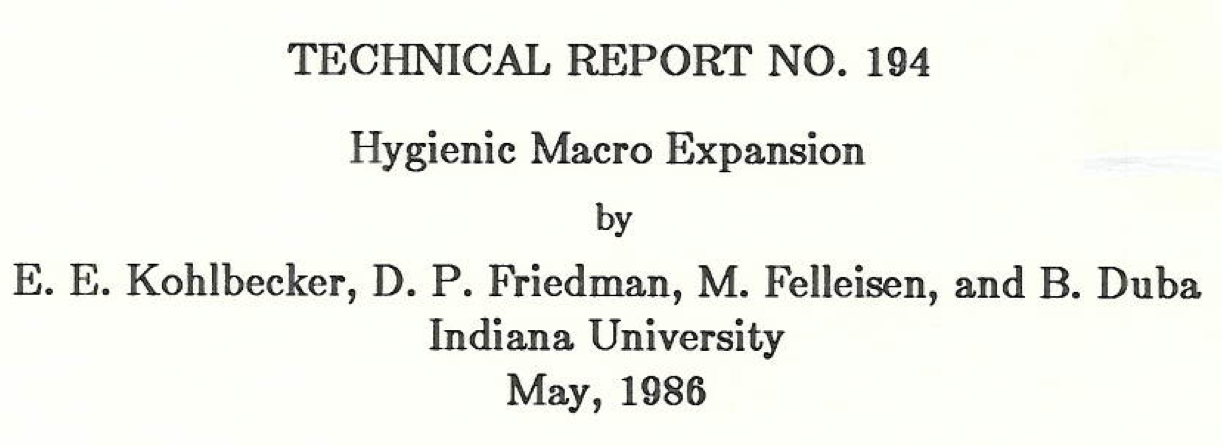
\includegraphics[height=4cm]{hygiene.png}
\end{center}
\end{frame}

\begin{frame}[fragile]{Hygiene in action}
\begin{beforeblock}
scala> val list = q"List(1, 2, 3)"
list: universe.Tree = List(1, 2, 3)

scala> tb.eval(q"val List = 42; \$list")
compilation has failed: Int does not take parameters
\end{beforeblock}
\begin{afterblock}
scala> val list = q"List(1, 2, 3)"
list: meta.Tree = List(1, 2, 3)

scala> q"val List = 42; \$list".eval
res1: Any = List(1, 2, 3)
\end{afterblock}
\end{frame}

\sectionframe{Tree design}

\begin{frame}[fragile]{Trees are now comprehensive}
\begin{beforeblock}
scala> q"for (i <- List(1, 2, 3)) println(i)"
res0: universe.Tree = List(1, 2, 3).foreach(i => println(i))
\end{beforeblock}
\pause
\begin{afterblock}
scala> q"for (i <- List(1, 2, 3)) println(i)"
res1: meta.Term = for (i <- List(1, 2, 3)) println(i)
\end{afterblock}
\end{frame}

\begin{frame}{Trees are now comprehensive}
\begin{itemize}
\item In \texttt{scala.meta}, we keep all the information about the program
\item Nothing is desugared (e.g. \texttt{for} loops or string interpolations)
\item Nothing is thrown away (e.g. comments or formatting details)
\end{itemize}

\end{frame}
\begin{frame}[fragile]{Trees are now strongly-typed}
\begin{beforeblock}
case class Apply(fun: Tree, args: List[Tree])
\end{beforeblock}
\begin{afterblock}
@ast class Apply(fun: Term, args: Seq[Arg])
\end{afterblock}
\end{frame}

\begin{frame}[fragile]{In \texttt{scala.reflect}}
\begin{semiverbatim}
scala> val List = tq"_root_.scala.List"
List: universe.Select = _root_.scala.List

scala> val list = q"\$List(1, 2, 3)"
list: universe.Tree = _root_.scala.List(1, 2, 3)

scala> toolbox.typecheck(list)
s.t.r.ToolBoxError: type scala.List is not a value
  at s.t.r.ToolBoxFactory\$...apply(ToolBoxFactory.scala:178)
  at s.t.r.ToolBoxFactory\$...apply(ToolBoxFactory.scala:170)
  at s.t.r.ToolBoxFactory\$...apply(ToolBoxFactory.scala:148)
  ...
\end{semiverbatim}
\end{frame}

\begin{frame}[fragile]{In \texttt{scala.meta}}
\begin{semiverbatim}
scala> val List = t"_root_.scala.List"
List: meta.Type = _root_.scala.List

scala> val list = q"\$List(1, 2, 3)"
<console>:27: error: type mismatch;
 found   : Type
 required: Term
              val list = q"\$List(1, 2, 3)"
                            ^
\end{semiverbatim}
\end{frame}

\begin{frame}[c, fragile]{Boromir has certain doubts about \texttt{scala.reflect}}
\begin{center}
% http://www.cs.uni.edu/~wallingf/teaching/cs3540/sessions/session26.html

\includegraphics[height=6cm]{mutable-state.jpg}
\end{center}
\end{frame}

\begin{frame}[fragile]{Trees are now immutable}
\begin{beforeblock}
abstract class Tree \{
  private[this] var rawtpe: Type = \_
  def tpe: Type = rawtpe
  def setType(tp: Type): this.type = \{ rawtpe = tp; this \}
  ...
\}
\end{beforeblock}
\pause
\begin{afterblock}
implicit class SemanticTermOps(val term: Term) extends AnyVal \{
  @hosted def tpe: Type = ...
\}
\end{afterblock}
\end{frame}

\sectionframe{Anytime metaprogramming}

\begin{frame}{Flavors of metaprogramming}
\begin{itemize}
\item Compile-time metaprogramming (macros)
\item Runtime metaprogramming (runtime reflection, toolboxes)
\item Some-time metaprogramming (IDEs, incremental compilation, linters)
\end{itemize}
\end{frame}

\begin{frame}{Flavors of environments}
\begin{itemize}
\item Scala compiler (\texttt{scala-reflect.jar} and \texttt{scala-compiler.jar})
\item IntelliJ IDEA (a very own implementation of Scala's typechecker)
\item Scala IDE (Scala compiler running in a funny mode)
\item SBT (A tiny compiler plugin + a very own analysis infrastructure)
\item DIY (Just have some Scala sources and need to find something out)
\end{itemize}
\end{frame}

\begin{frame}{Too complicated again!}
\begin{itemize}
\item Typechecking and evaluation kind of work at runtime, but not quite
\item Macros work at compile time, but only in a separate project
\item Macros seem to work in IntelliJ, but they actually don't
\end{itemize}
\end{frame}

\begin{frame}{With \texttt{scala.meta} it's no longer a problem}
\vskip35pt
\begin{center}
\text{\Large{Demo!}}
\end{center}
\end{frame}

\begin{frame}[c, fragile]{But how is this supposed to work?!}
% http://www.quickmeme.com/meme/2dq8
\begin{center}

\includegraphics[height=7cm]{noway.jpg}
\end{center}
\end{frame}

\begin{frame}{But how is this supposed to work?!}
\begin{itemize}
\item Macros are known to be just bytecode invoked by reflection
\item But when macros aren't compiled yet, there's no bytecode
\item Therefore having macros work in the same file would be most unusual
\item This merits an explanation
\end{itemize}
\end{frame}

\begin{frame}{Explanation, in a nutshell}
\begin{itemize}
\item With \texttt{scala.meta}, we have principled tools for metaprogramming
\item This makes it possible to make macros principled
\item When macros become a proper abstraction, all becomes much better
\end{itemize}
\end{frame}

\begin{frame}{Explanation, part 1: Clear requirements for all hosts}
\begin{itemize}
\item A standalone, independent metaprogramming interface
\item Built on simple, strongly-typed and immutable foundation
\item With clear and concise host API
\item Prototype implementations for \texttt{scalac} and IntelliJ
\end{itemize}
\end{frame}

\begin{frame}[c, fragile]{Explanation, part 1: Clear requirements for all hosts}
% source?
\begin{center}

\includegraphics[height=6cm]{score.png}
\end{center}
\end{frame}

\begin{frame}{Explanation, part 2: Equal opportunities for all hosts}
\begin{itemize}
\item With our plugin enabled, \texttt{scalac} saves all ASTs after typer
\item This means that full info about any program is available at any time
\item No information is lost anymore (e.g. signatures of local definitions)
\item The overhead is actually quite reasonable (e.g. compressed \emph{untyped} ASTs of scala-library.jar are less than 15\% of the bytecodes)
\end{itemize}
\end{frame}

\begin{frame}{Explanation, part 3: Brave new world!}
\begin{itemize}
\item Easy access to all ASTs enables a lot of interesting things
\item One of them is host-independent AST interpretation
\item That's exactly what we're using to lift the precompilation restriction
\end{itemize}
\end{frame}

\begin{frame}[c, fragile]{Anytime metaprogramming}
% http://memegenerator.net/instance/50705398
\begin{center}

\includegraphics[height=7.5cm]{much-meta.jpg}
\end{center}
\end{frame}

\begin{frame}{Automatic code rewriting tool}
\begin{itemize}
\item As of late, there have been talks about deprecating procedure syntax
\item But it's so common that warnings are only emitted under \texttt{-Xfuture}
\item It would be nice to have an automatic migration tool for this!
\end{itemize}
\end{frame}

\begin{frame}{Automatic code rewriting tool}
\begin{itemize}
\item Unfortunately existing \texttt{scalac} functionality isn't quite fit for that
\item Wheels are reinvented in order to do robust parsing and prettyprinting
\item With \texttt{scala.meta}, this become very simple!
\end{itemize}
\end{frame}

\begin{frame}[fragile]{Automatic code rewriting tool}
\begin{semiverbatim}
some/project\$ sbt meta
[info] Loading project definition...
[info] Starting scala interpreter...
\pause
> project
res0: Project = Project(List("scalameta/package.scala",
"scalameta/Trees.scala", "scalameta/semantic/Hosts.scala"..))
\pause
> project.rewrite \{
|   case q"..\$mods def \$nme[..\$tps](...\$pss) \{ ..\$body \}" =>
|   q"..\$mods def \$nme[..\$tps](...\$pss): Unit = \{ ..\$body \}"
| \}.persist
res1: Project = Project(List("scalameta/package.scala",
"scalameta/Trees.scala", "scalameta/semantic/Hosts.scala"..))
\end{semiverbatim}
\end{frame}

\sectionframe{Wrapping up}

\begin{frame}{Brought to you by the Palladium team}
This project is brought to you by the Palladium team.\\
Thank you very much, folks, for making this presentation possible!

\begin{tabular}{p{0.4\textwidth}p{0.5\textwidth}}
\begin{itemize}
\itemsep0.5em
\item Uladzimir Abramchuk
\item Igor Bogomolov
\item Eugene Burmako
\item Mathieu Demarne
\item Martin Duhem
\item Adrien Ghosn
\item Mikhail Mutcianko
\end{itemize} &
\begin{itemize}
\itemsep0.5em
\item Dmitry Naydanov
\item Artem Nikiforov
\item Vladimir Nikolaev
\item Alexander Podkhalyuzin
\item Jatin Puri
\item Denys Shabalin
\end{itemize} \\
\end{tabular}
\end{frame}

\begin{frame}{What we've seen today}
\begin{itemize}
\item Built on a simple principle that everything is a tree
\item And designed in strongly-typed and fully immutable style
\item \texttt{scala.meta} is a clean and portable metaprogramming toolkit
\item Public preview is coming this fall
\item But some results are available right now (e.g. sbt improvements)
\end{itemize}
\end{frame}

\begin{frame}[c, fragile]{Public preview coming this fall at \href{http://scalameta.org/}{scalameta.org}!}
\begin{center}
% http://www.movieviral.com/wp-content/uploads/2009/04/nx01.jpg

\includegraphics[height=7.5cm]{nx01-therealthing.jpg}\\
\end{center}
\end{frame}

\end{document}